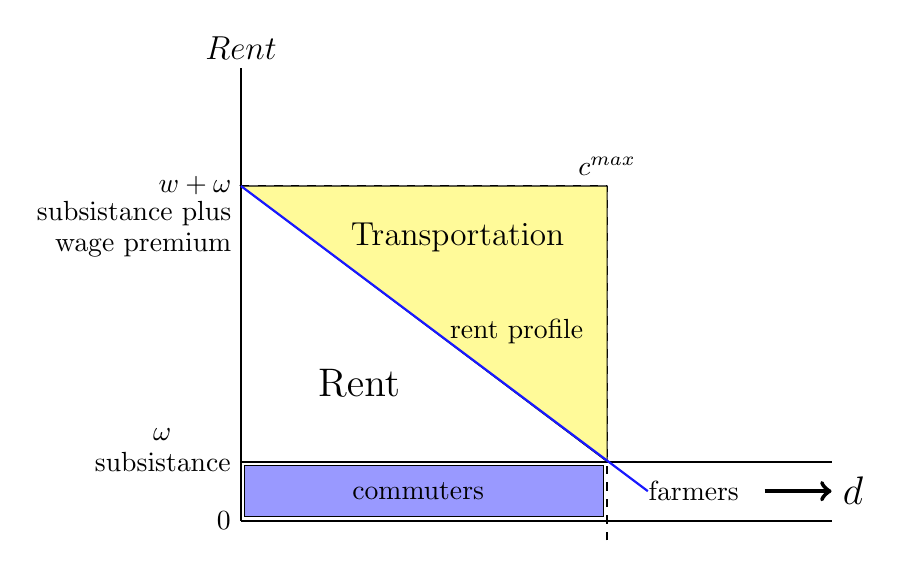
\begin{tikzpicture}[scale=.5]
\def\bndmax{5}        
\def\bndmin{0.2}
\def \n {10}  % height of y axis
\def \d {15}  % length  of x axis
\def \t {.75}  %  cost of transportation per unit x
\def \th {1}   %
\def \w {7}    %  wage premium
\def \om{1.5}%  omega =rural wage Zero for urban population
\def \azero{2}
\def \aprime {-.0}	
\tikzset{func/.style={thick,color=blue!90}}	
\draw [thick] (0,-\om) --(\d,-\om);  			% Zero for rural population
\draw [thick] (0,-\om)node[left]{$0$} --(0,\n);	% Y axis
\node at (0,\n+0.5){\large$Rent$};

\draw [thick] (0,0)node[left]{subsistance}--(\d,0);
\node a t(-2,.7) {$\omega$};
\node[left] at (0,\w){$w+\omega$};
\node[left] at (0,\w-.7){subsistance plus};
\node[left] at (0,\w-1.5){wage premium};	
\draw [dashed, thick](9.3,-2)-- (9.3,\w)node[above]{$c^{max}$};
\draw [dashed, thick](0,\w)-- (9.3,\w);
% solid color for commuters
\draw[fill=blue!40] (0.1,-0.1) rectangle (9.2,-\om+.1);
\draw[fill=yellow!40] (9.30,7.) -- (0,7)--(9.30,0.)--cycle;% Rent \w-.2
\draw[func,domain=0:\w/\t+1] plot [samples=200] (\x,{\w-\t*\x});
\node at (5.5,5.7){\large Transportation};
\node at (7,3.3){rent profile};		%Rent Profile	
\node at (3.,2){\Large Rent}; 		%Rent 
\node at (4.5,-\om/2){commuters};
\node at (11.5,-\om/2){farmers};
\draw [ ultra thick, ->](13.3,-\om/2)--(15, -\om/2)node [right] {\Large $d$};
\end{tikzpicture}